 \documentclass[parskip=half]{scrartcl}
\usepackage{amsmath}
\usepackage{booktabs}
\usepackage[T1]{fontenc}
\usepackage{graphicx}
\usepackage{natbib}
\usepackage{tikz}
\usetikzlibrary{shapes,arrows,decorations.pathmorphing,calc}


\bibliographystyle{agufull08}

\newcommand{\changefont}[3]{\fontfamily{#1} \fontseries{#2} \fontshape{#3} \selectfont}

%% diverser Plunder
\renewcommand{\refname}{Literature}
%\renewcommand{\appendixname}{Appendix}
%\newcommand{\tnoocomment}[1]{\marginpar{\psshadowbox[framearc=0.3,shadowsize=2pt]{\footnotesize #1}}}
\newcommand{\tnoocomment}[1]{\marginpar{\fbox{\footnotesize #1}}}
\newcommand{\tinu}[1]{\marginpar{\fbox{\footnotesize #1}}}
\newcommand{\todo}[1]{\fbox{#1}}
\newcommand{\idea}[1]{\marginpar{\fbox{\parbox{2.2cm}{\tiny #1}}}}

%% commands to facilitate units and temperature
\newcommand{\unit}[1]{\ensuremath{\,\mathrm{#1}}}
\newcommand{\s}[1]{\ensuremath{\,\mathrm{#1}}}
\newcommand{\cels}[1]{\ensuremath{#1^{\circ}\,\mathrm{C}}}


\newcommand{\hbe}{\hat{\mathbf{e}}}
%\newcommand{\define}[1]{{\textbf{#1}}\marginpar{\psshadowbox[framearc=0.3,shadowsize=2pt]{\footnotesize #1}}}
\newcommand{\define}[1]{{\textbf{#1}}\marginpar{\fbox{\footnotesize #1}}}
\newcommand{\epsdot}{\dot{\varepsilon}}
\newcommand{\bsigma}{\mbox{\boldmath$\sigma$\unboldmath}}
\newcommand{\bepsdot}{\mbox{\boldmath$\epsdot$\unboldmath}}


% Some useful commands (from ELB)
\newcommand{\bD}{\mathbf{D}}
\newcommand{\bbf}{\mathbf{f}}
\newcommand{\bF}{\mathbf{F}}
\newcommand{\bg}{\mathbf{g}}
\newcommand{\bn}{\mathbf{n}}
\newcommand{\bq}{\mathbf{q}}
\newcommand{\bT}{\mathbf{T}}
\newcommand{\bu}{\mathbf{u}}
\newcommand{\bU}{\mathbf{U}}
\newcommand{\bv}{\mathbf{v}}

\newcommand{\ddx}[1]{\ensuremath{\frac{\partial #1}{\partial x}}}
\newcommand{\ddy}[1]{\ensuremath{\frac{\partial #1}{\partial y}}}
\newcommand{\ddz}[1]{\ensuremath{\frac{\partial #1}{\partial z}}}
\newcommand{\ddt}[1]{\ensuremath{\frac{\partial #1}{\partial t}}}

\newcommand{\DDt}[1]{\ensuremath{\frac{d #1}{d t}}}

\newcommand{\Div}{\nabla\cdot}
\newcommand{\eps}{\epsilon}
\newcommand{\grad}{\nabla}
\newcommand{\half}{\frac{1}{2}}
\newcommand{\trace}{\operatorname{tr}}

\newcommand{\rinv}{\frac{1}{r}}
\newcommand{\ar}{r^{-1}\alpha}
\newcommand{\stress}{\ensuremath{\text{\Large$\sigma$\normalsize}}}
\newcommand{\devstress}{\ensuremath{\text{\Large$\tau$\normalsize}}}


% ---------------------------------------------------------------------------------------
% definition of header and footer
% ---------------------------------------------------------------------------------------

\usepackage[automark,headsepline,footsepline]{scrpage2}
\clearscrheadings	% definition headings loeschen
\ihead{Thermodynamics of Glaciers}
\cfoot{\pagemark}
\setkomafont{pagehead}{\normalfont}	% font kopfzeile
\setkomafont{pagenumber}{\normalfont\rmfamily}	% font kopfzeile zahlen




% ---------------------------------------------------------------------------------------
% Koma-Script - Settings
% ---------------------------------------------------------------------------------------
\addtokomafont{caption}{\small}
\setkomafont{captionlabel}{\sffamily\bfseries}
% \setkomafont{caption}{\sffamily}
\setcapindent{1em}

\pagestyle{scrheadings}



\begin{document}
\title{Thermodynamics of Glaciers\\[.5em]
\rule[1.em]{\textwidth}{2pt}}
\subtitle{McCarthy Summer School 2016}

\date{June 2016}

\author{
  \small Andy Aschwanden\\[-.5em] 
 \small University of Alaska Fairbanks, USA}


\maketitle

\textbf{Note}: This script is largely based on the \emph{Physics of
Glaciers I} lecture notes by Martin L\"uthi and Martin Funk, ETH
Zurich, Switzerland, with additions from \cite{GreveBlatter_disg},
\cite{Gusmeroli2010} and \cite{Aschwanden2012}.

\vspace{1em}

In glaciers thermodynamics, glaciers are divided into three categories, depending on their thermal structure:
%
\begin{description}
\item[Cold] The temperature of the ice is below the pressure melting
temperature throughout the glacier, except for maybe a thin surface
layer.
\item[Temperate] The whole glacier is at the pressure melting
temperature, except for seasonal freezing of the surface layer.
\item[Polythermal] Some parts of the glacier are cold, some temperate.
Usually the highest accumulation area, as well as the upper part of an
ice column are cold, whereas the surface and the base are at melting
temperature.
\end{description}
%
The knowledge of the distribution of temperature in glaciers and ice
sheets is of high practical interest:
%
\begin{itemize}\itemsep0ex
\item A temperature profile from a cold glacier contains information
on past climate conditions.
\item Ice deformation is strongly dependent on temperature
(temperature dependence of the rate factor $A$ in Glen's flow law).
\item The routing of meltwater through a glacier is affected by ice
temperature.  Cold ice is essentially impermeable, except for discrete
cracks and channels.
\item If the temperature at the ice-bed contact is at the pressure
melting temperature the glacier can slide over the base.
\item Wave velocities of radio and seismic signals are temperature
dependent. This affects the interpretation of ice depth soundings.
\end{itemize}

The distribution of temperature in a glacier depends on many factors.
Heat sources are on the glacier surface, at the glacier base and
within the body of the ice.  Heat is transported through a glacier by
conduction (diffusion), is advected with the moving ice, and is
convected with water or air flowing through cracks and channels.  Heat
sources within the ice body are (Figure~\ref{fig:energy-sources})
%
\begin{itemize}\itemsep0ex
\item dissipative heat production (internal friction) due to ice
deformation,
\item frictional heating at the glacier base (basal motion)
\item frictional heating of flowing water at englacial channel walls,
\item release or consumption of (latent) heat due to freezing and
melting.
\end{itemize}
%
The importance of the processes depends on the climate regime a
glacier is subjected to, and also varies between different parts of
the same glacier.


\section{Energy balance equation}
\label{sec:energy-balance}

The energy balance equation for internal energy $U$ is an
advection-diffusion-production equation which in a spatially fixed
(Eulerian) reference frame is given by
\begin{equation}
  \label{eq:energy-balance} \rho \left(\ddt{U} + \underbrace{\bv \cdot
\grad U}_{\textrm{advection}}\right) = - \underbrace{\Div
\bq}_{\textrm{diffusion}} + \underbrace{Q}_{\textrm{production}},
\end{equation} where $\rho$ is density and $q$ is a non-advective
energy flux. Note that, strictly speaking, internal energy is not a
conserved quantity, only the sum of internal energy and kinetic energy is
conserved.
%

\section{Cold ice}

If ice is below the pressure melting point, we can replace internal
energy $U=c\,T$ with temperature $T$:
\begin{equation}
  \label{eq:temperature-equation} \rho c\left(\ddt{T} + \underbrace{\bv
\cdot \grad T}_{\textrm{advection}}\right) = \underbrace{\nabla
k\nabla T}_{\textrm{diffusion}} +
\underbrace{Q}_{\textrm{production}},
\end{equation} where specific heat capacity $c$ and thermal
conductivity $k$ are given in Table \ref{tab:thermal-properties}. In
general, specific heat capacity and thermal heat conductivity are
functions of temperature \citep[e.g.][]{Ritz1987},
\begin{equation}
  \label{eq:specific-heat} c(T) = (146.3 + 7.253 T
[\text{K}])\,\text{J}\,\text{kg}^{-1}\,\text{K}^{-1}
\end{equation} and
\begin{equation}
  \label{eq:heat-conductivity} k(T) = 9.828 e^{-0.0057 T
[\text{K}]}\,\text{W}\,\text{m}^{-1}\,\text{K}^{-1}.
\end{equation}

\begin{figure} \centering
   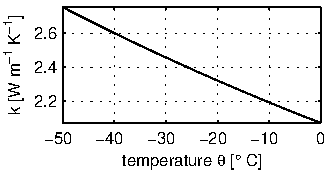
\includegraphics[width=7cm]{figures/k} \hfill
   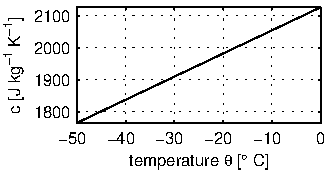
\includegraphics[width=7cm]{figures/c}
   \caption{Heat conductivity $k$ (left) and specific heat $c$ (right)
for the temperature range from \cels{-50} until \cels{0}. After
\cite{Ritz1987}.}
\end{figure}
%
For constant thermal conductivity $k$ and in one dimension (the
vertical direction $z$ and vertical velocity $w$) the energy balance
equation (\ref{eq:temperature-equation}) reduces to
%
\begin{equation}
 \label{eq:heat-diffusion-advection-1d} \rho\, c \left(\ddt{T} + w
\ddz{T}\right) = k\, \frac{\partial^2T}{\partial z^2} + P.
\end{equation}

The heat production (source term) $P$ can be due to different
processes (see Figure~\ref{fig:energy-sources}):\\[-1em]
%
\begin{description}
\item[Dissipation] In viscous flow the \emph{dissipation}
\index{dissipation} due to ice deformation (heat release due to
internal friction, often called strain heating) is
$P=\mathrm{tr}({\bepsdot\bsigma})= \epsdot_{ij}\sigma_{ji}$, where
$\bepsdot$ and $\bsigma$ are the strain rate tensor and the stress
tensor, respectively..  Because usually the shearing deformation
dominates glacier flow
 \begin{equation*} P_{\text{def}} \simeq 2
\;\epsdot_{xz}\sigma_{xz}\,.
 \end{equation*}
\item[Sliding friction] The heat production is the rate of loss of
potential energy as an ice column of thickness $H$ moves down slope.
If all the frictional energy is released at the bed due to sliding
with basal velocity $u_b$,
 \begin{equation*} P_{\text{friction}} = \tau_bu_b \sim \rho g H
\tan\beta \, u_b \,,
 \end{equation*} where $\tau_b$ is basal shear stress and $\beta$ is
the bed inclination.
\item[Refreezing of meltwater] Consider ice that contains a volume
fraction $\omega$ of water. If a freezing front is moving with a
velocity $v_\text{freeze}$ relative to the ice, the rate of latent
heat production per unit area of the freezing front is
 \begin{equation*} P_{\text{freeze}} = v_\text{freeze} \,\omega \rho_w
L.
 \end{equation*}
\end{description}

  \begin{figure} \centering
    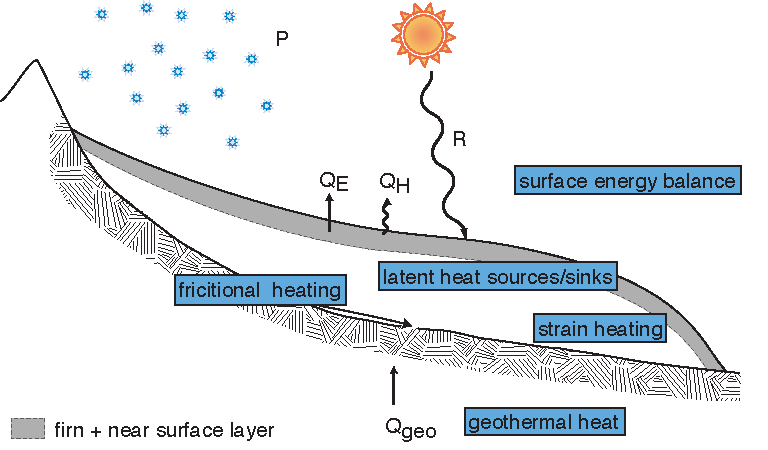
\includegraphics[width=12cm]{figures/glacier_thermodynamics}
    \caption{Sources for heat production}
    \label{fig:energy-sources}
  \end{figure}


\begin{table}[thb] \centering
 \begin{tabular}[h]{lcrl} \toprule Quantity & Symbol & Value & Unit\\
\midrule
Density of ice & $\rho_i$ & $\sim 917$ & $\unit{kg}\unit{m}^{-3}$ \\ 
Specific heat capacity of water & $c_w$ & $4182$ & $\unit{J}\unit{K}^{-1}\unit{kg}^{-1}$ \\ Specific heat capacity of ice & $c_i$ & $2093$ &
$\unit{J}\unit{K}^{-1}\unit{kg}^{-1}$ \\ 
Thermal conductivity of ice (at \cels{0}) & $k$ & $2.1$ & $ \unit{W}\unit{m}^{-1}\unit{K}^{-1}$ \\
Thermal diffusivity of ice (at \cels{0}) & $\kappa$ & $1.09\cdot
10^{-6}$ & $ \unit{m}^{2}\unit{s}^{-1}$ \\ 
Latent heat of fusion (ice/water) & $L$ & $333.5$ & $\unit{kJ}\unit{kg}^{-1}$\\
\multicolumn{4}{l}{Depression of melting temperature
(Clausius-Clapeyron constant)} \\ 
\hspace{2ex}- pure ice and air-free
water & $\gamma$ & $0.0742$ & $ \unit{K}\unit{MPa}^{-1}$ \\
\hspace{2ex}- pure ice and air-saturated water & $\gamma$ & $0.098$ &
$ \unit{K}\unit{MPa}^{-1}$ \\ \addlinespace[1ex] \bottomrule
\end{tabular}
\caption{Thermal properties of ice and water.}
\label{tab:thermal-properties}
\end{table}


\subsection{Steady temperature profile}
\label{sec:steady-temp-profile}

The simplest case is a vertical steady state temperature profile
(Eq.~\ref{eq:heat-diffusion-advection-1d} without time derivative) in
stagnant ice ($w=0$) without any heat sources ($P=0$), and with
constant thermal conductivity $k$.  The heat flow equation
(\ref{eq:heat-diffusion-advection-1d}) then reduces to the diffusion
equation
%
\begin{equation}
 \label{eq:diffusion-1d} \frac{\partial^2T}{\partial z^2} = 0.
\end{equation}
%
Integration with respect to $z$ gives
%
\begin{equation}
 \label{eq:diffusion-1d-1int} \frac{dT}{d z} = Q := k G
\end{equation}
%
where $G = \nabla T$ is the (constant) temperature
gradient. Integrating again leads to
%
\begin{equation}
 \label{eq:diffusion-1d-2int} T(z) = G z + T(0) = \frac{Q}{k} z +
T(0).
\end{equation}
%
Ice temperature changes linearly with depth.  Choosing for example a
temperature gradient of $G=1\unit{K}/ 100\unit{m} =
0.01\unit{K}\unit{m}^{-1} = 10 \unit{mK}\unit{m}^{-1}$ gives a heat
flux of $Q = kG = 0.021\unit{W} \unit{m}^{-2} = 21\unit{mW}
\unit{m}^{-2}$.  For comparison, typical geothermal fluxes are $40-
120 \unit{mW} \unit{m}^{-2}$ but can reach up to $1000 \unit{mW} \unit{m}^{-2}$ \citep{Fahnestock2001a}. 

To transport a geothermal flux of $80 \unit{mW} \unit{m}^{-2}$ through
a glacier of $200\unit{m}$ thickness, the surface temperature has to
be $8\unit{K}$ lower than the temperature at the glacier base.

The above calculations (partly) explain why there can be water at the
base of the Greenland and Antarctic ice sheets.  Under an ice cover of
$3000\unit{m}$ and at surface temperatures of \cels{-50} (in
Antarctica), only a heat flux of $Q=k \cdot 50\unit{K}/3000\unit{m}=
35\unit{mW}\unit{m}^{-2}$ can be transported away.  Notice that
horizontal and vertical advection change this result considerably.


\subsection{Ice temperature close to the glacier surface}
\label{sec:ice-temp-surface}

The top $15\s{m}$ of a glacier (near surface layer,
Figure~\ref{fig:energy-sources}) are subject to seasonal variations of
temperature. In this part of the glacier \emph{heat flow} (\emph{heat
diffusion}) is dominant.  If we neglect advection we can rewrite
Equation (\ref{eq:heat-diffusion-advection-1d}) to obtain the well
known \emph{Fourier law} of heat diffusion
%
\begin{equation}
 \label{eq:heat-flow-1d} \ddt{T} = \kappa \,
\frac{\partial^2T}{\partial h^2}
\end{equation}
%
where $h$ is depth below the surface, and $\kappa=k/(\rho C)$ is the
\emph{thermal diffusivity} of ice.  To calculate a temperature profile
and changes with time we need boundary conditions.  Periodically
changing boundary conditions at the surface such as day/night and
winter/summer can be approximated with a sine function.  At depth we
assume a constant temperature $T_0$
%
\begin{align}
 \label{eq:heat-flow-1d-bound} T(0,t) &= T_0 + \Delta T_0 \cdot
\sin(\omega t)\,, \notag\\ T(\infty,t) &= T_0\,.
\end{align}
%
$T_0$ is the mean surface temperature and $\Delta T_0$ is the
amplitude of the periodic changes of the surface temperature.  The
duration of a period is $2\pi/\omega$.  The solution of Equation
(\ref{eq:heat-flow-1d}) with the boundary condition
(\ref{eq:heat-flow-1d-bound}) is
%
\begin{equation}
 \label{eq:heat-flow-1d-solution} T(h,t) = T_0 + \Delta T_0
\exp\left(-h \sqrt{\frac{\omega}{2\kappa}}\right) \sin\left(\omega t -
h \sqrt{\frac{\omega}{2\kappa}}\right).
\end{equation}
%
The solution is plotted for realistic values of $T_0$ and $\Delta T$
on Colle Gnifetti ($4550\unit{m} \unit{a.s.l.}$, Monte Rosa, Valais).
Notice that full ice density has been assumed for the plot, instead of
a firn layer with strongly changing thermal properties, and vertical
advection is neglected.
%
\begin{figure}[htbp] \centering
 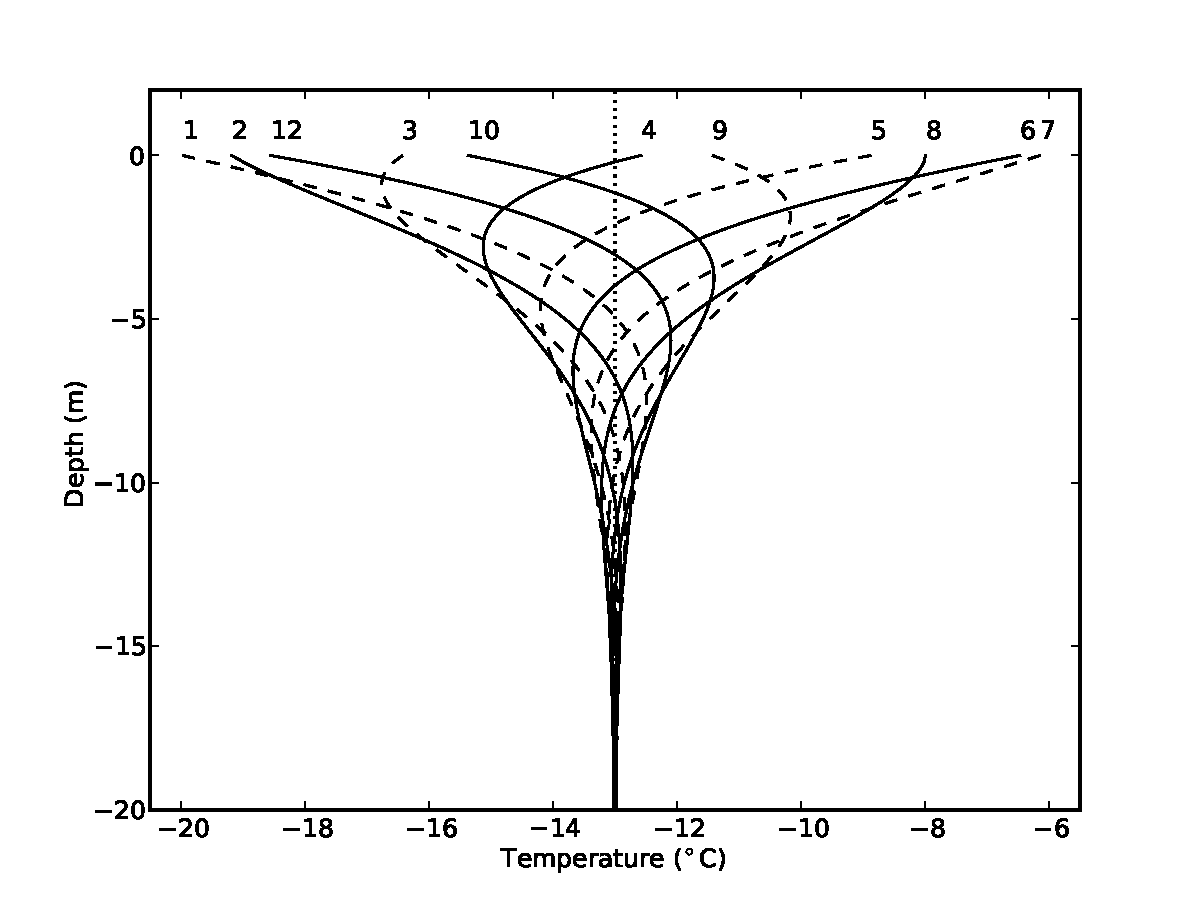
\includegraphics[height=10.cm]{figures/temp-variation}
 \caption{Variation of temperature with depth for the conditions at
Colle Gnifetti.  Numbers next to curves indicate months (1 corresponds
to January). }
 \label{fig:water}
\end{figure}

The solution (Eq.~\ref{eq:heat-flow-1d-solution}) has some noteworthy
properties
%
\begin{itemize}
\item[a)] The amplitude varies with depth $h$ as
%
 \begin{equation}
   \label{eq:temp-depth-amplitude} \Delta T(h) = \Delta T_0
\exp\left(-h \sqrt{\frac{\omega}{2\kappa}}\right)
 \end{equation}
\item[b)] The temperature $T(h,t)$ has an extremum when
 \begin{equation*} \sin\left(\omega t - h
\sqrt{\frac{\omega}{2\kappa}}\right) = \pm 1 \qquad \Rightarrow \qquad
\omega t - h \sqrt{\frac{\omega}{2\kappa}} = \frac{\pi}{2}
 \end{equation*} and therefore
 \begin{equation}
   \label{eq:temp-depth-maximum} t_{\textrm{max}} =
\frac{1}{\omega}\left( \frac{\pi}{2} + h \sqrt{\frac{\omega}{2\kappa}}
\right)
 \end{equation} The phase shift is increasing with depth below the
surface.
\item[c)] The heat flux $G(h,t)$ in a certain depth $h$ below the
surface is
%
 \begin{equation*} G(h,t) = -k\frac{\partial T}{\partial h} = %\cdots
\quad \text{\small (complicated formula that is easy to derive)}
 \end{equation*}
%
 For the heat flux $G(0,t)$ at the glacier surface we get
 \begin{equation*} G(0,t) = \Delta T_0 \sqrt{\omega \rho\, c\,k}\,
\sin\left(\omega t + \frac{\pi}{4}\right)
 \end{equation*}
%
 $G(0,t)$ is maximal when
%
 \begin{align*} \sin\left(\omega t + \frac{\pi}{4}\right)=1
\qquad\Rightarrow \qquad \omega t + \frac{\pi}{4} = \frac{\pi}{2}
\qquad \Longrightarrow \qquad t_{\text{max}} = \frac{\pi}{4\omega}
 \end{align*}
%
 where $t_{\text{max}}$ is the time when the heat flux at the glacier
surface is maximum.
%
\begin{align*} &\text{Temperature:}& t_{\textrm{max}}&=
\frac{\pi}{2\omega}\\ &\text{Heat flux:} & t_{\textrm{max}} &=
\frac{\pi}{4\omega}
\end{align*}
%
The difference is $\pi/(4\omega)$ and thus $1/8$ of the period.  The
maximum heat flux at the glacier surface is $1/8$ of the period ahead
of the maximum temperature.  For a yearly cycle this corresponds to
1.5 months.
\item[d)] From the ratio between the amplitudes in two different
depths the heat diffusivity $\kappa$ can be calculated
 \begin{align*} \frac{\Delta T_2}{\Delta T_1} = \exp \left( (h_1-h_2)
\sqrt{\frac{\omega}{2\kappa}} \right) \qquad\Longrightarrow \qquad
\kappa = \frac{\omega}{2} \left(\frac{h_2-h_1}{\ln \frac{\Delta
T_2}{\Delta T_1}}\right)^2
  \end{align*}
\end{itemize}

There are, however, some restrictions to the idealized picture given
above
%
\begin{itemize}
\item The surface layers are often not homogeneous.  In the
accumulation area density is increasing with depth. Conductivity $k$
and diffusivity $\kappa$ are functions of density (and also
temperature).
\item In nature the surface boundary condition is not a perfect sine
function.
\item The ice is moving.  Heat diffusion is only one part, heat
advection may be equally important.
\item Percolating and refreezing melt water can drastically change the
picture by providing a source of latent heat (see below).
\end{itemize}
%
Superimposed on the yearly cycle are long term temperature changes at
the glacier surface.  These penetrate much deeper into the ice, as can
be seen from Equation (\ref{eq:temp-depth-amplitude}), since $\omega$
decreases for increasing forcing periods.

In spring or in high accumulation areas the surface layer of a glacier
consists of snow or firn.  If surface melting takes place, the water
percolates into the snow or firn pack and freezes when it reaches a
cold layer.  The freezing of $1\unit{g}$ of water releases sufficient
heat to raise the temperature of $160\unit{g}$ of snow by $1\unit{K}$.
This process is important to ``annihilate'' the winter cold from the
snow or firn cover in spring, and is the most important process
altering the thermal structure of high accumulation areas and of the
polar ice sheets.

\subsection{Advection -- diffusion}
\label{sec:advection-diffusion}

Close to the ice divides in the central parts of an ice sheet, the ice
velocity is mainly vertical down.  Under the assumptions of only
vertical advection, no heat generation, and a frozen base we can
calculate the steady state temperature profile with the simplified
Equation (\ref{eq:heat-diffusion-advection-1d})
%
\begin{equation}
 \label{eq:heat-diffusion-advection-1d-steady} \kappa \frac{d^2T}{d
z^2} = w(z) \frac{d T}{d z}
\end{equation}
%
The boundary conditions are
\begin{align*} \text{surface:} \qquad & z=H: &\qquad
\text{temperature}\;T_s = \text{const}\\ \text{bedrock:} \qquad & z=0:
&\qquad \text{heat flux}\;-k \left(\frac{dT}{dz}\right)_{B} = G =
\text{const}
\end{align*}
%
For the first integration we substitute $f = \frac{dT}{dz}$ so that
$\kappa f' = wf \; \Longrightarrow \; \frac{f' }{f} = \frac{1}{\kappa}
w$ with the solution
%
\begin{equation}
 \label{eq:8} \frac{dT(z)}{dz} = \left(\frac{dT}{dz}\right)_{B} \exp
\left( \frac{1}{\kappa} \int_0^z w(z)\, dz \right)\,.
\end{equation}
%
Now we make the assumption that the vertical velocity is $w(z) = -b
z/H$, with the vertical velocity at the surface equal to the net mass
balance rate $w_{s} = -\dot{b}$.  With the definition $l^2 := 2\kappa
H /\dot{b}$ we get
%
\begin{equation}
 \label{eq:10} T(z) - T(0) = \left(\frac{dT}{dz}\right)_{B} \int_0^z
\exp \left(-\frac{z^2}{l^2} \right) \,dz
\end{equation}
%
which has the solution
%
\begin{equation}
 \label{eq:11} T(z) - T_s = \frac{\sqrt\pi}{2} l
\left(\frac{dT}{dz}\right)_{B} \left[ {\textrm{erf}} \left(
\frac{z}{l} \right) - {\textrm{erf}} \left( \frac{H}{l} \right)
\right]\,.
\end{equation}
%
The so-called \emph{error function} is tabulated and implemented in
any mathematical software (usually as \texttt{erf}), and is defined as
%
\begin{equation*}
 \label{eq:12} {\textrm{erf}}(x) = \frac{2}{\sqrt{\pi}} \int_0^x
\exp(-x^2) \, dx.
\end{equation*}

We now introduce the useful definition of the \emph{P{\'e}clet Number}
$\text{Pe} = w H/\kappa$ which is a measure of the relative importance
of advection and diffusion.  The shape of the temperature profiles in
Figure \ref{fig:advection-diffusion} only depends on the P{\'e}clet
Number.  Depth and temperature can be scaled by the dimensionless
variables
%
\begin{align*} &\text{scaled distance above bed} & \xi &=
\frac{z}{H}\,,\\ &\text{scaled temperature} & \Theta &= \frac{k
(T-T_s)}{G H}\,.\\
\end{align*}
%
\begin{figure}[tbhp] \centering
 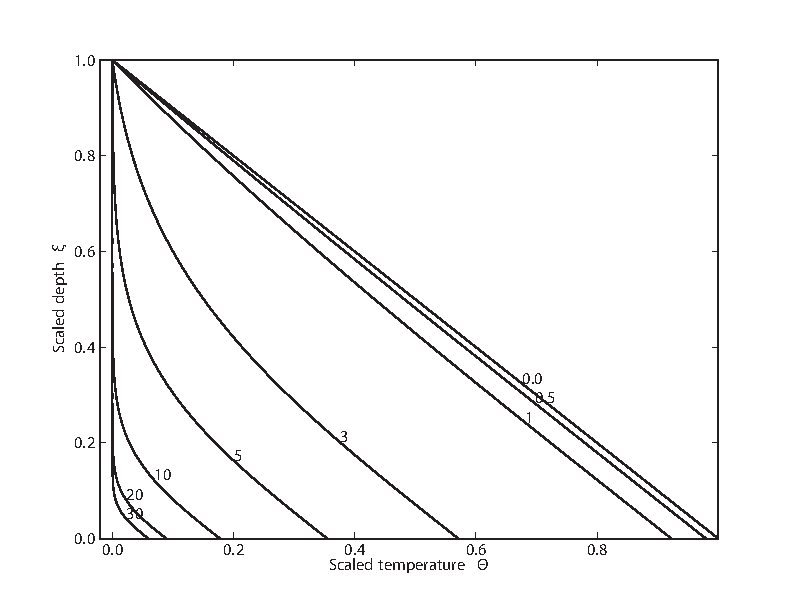
\includegraphics[width=0.9\textwidth]{figures/advection-diffusion}
  \caption{Dimensionless steady temperature profiles in terms of the
dimensionless variables $\xi$ and $\Theta$ for various values of the
P{\'e}clet number $\mathrm{Pe}$ (next to curves). }
   \label{fig:advection-diffusion}
\end{figure}


\subsection{Cold glaciers}
\label{sec:cold-glaciers}

In cold glaciers heat flow is driven by temperature gradients.
Usually the base is warmest due to dissipation, friction and
geothermal heat.  This has the consequence that heat is flowing from
the base into the ice body, warming up the ice.  Advection of warm or
cold ice strongly influences local ice temperature. Cold glaciers
exist in the McMurdo Dry Valleys in Antartica and at high altitudes at
lower latitudes.

In the Alps, for example, cold glaciers were observed at altitudes
above $3900\unit{m}\unit{a.s.l.}$.  The most famous of these is Colle
Gnifetti ($4550 \unit{m}\unit{a.s.l.}$), the highest accumulation
basin of the Gorner-/Grenzgletscher system.  At temperatures of about
\cels{-13} the ice conserves atmospheric conditions such as impurities
and air bubbles.  Surface melting only takes place on exceptionally
hot days and leads to formation of ice lenses.  Many ice cores have
been drilled on Colle Gnifetti and were investigated in the laboratory
to obtain the climate history of central Europe.

Figure \ref{fig:colle-profiles} shows two temperature profiles
measured in boreholes $200\unit{m}$ apart on the same flow line on
Colle Gnifetti.  In the absence of advection and density gradients,
one would expect straight steady state temperature profiles.  The
unequal curvature of the modeled steady state profiles
(Fig.~\ref{fig:colle-profiles}a) is due to firn density and different
advection regimes.  This shows that the interpretation of temperature
profiles to deduce past climate can be quite tricky.

The marked bend towards warmer temperature at $30\unit{m}$ depth is
due to changing surface temperatures.  Numerical modeling showed that
the temperature increase by \cels{1} around 1990 is mainly responsible
for this feature (the profiles were measured in 1995/96; in 1982 the
transient profiles looked like the steady state configuration).

\begin{figure}[p] \centering
 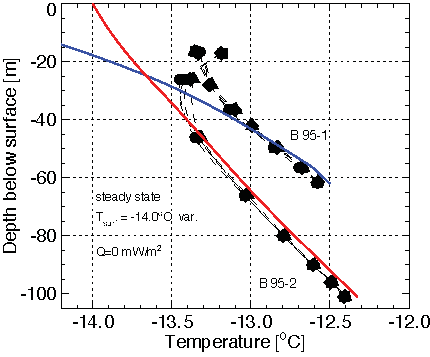
\includegraphics[width=0.49\textwidth]{figures/c_temp_steady_var_k32}
\hfill
   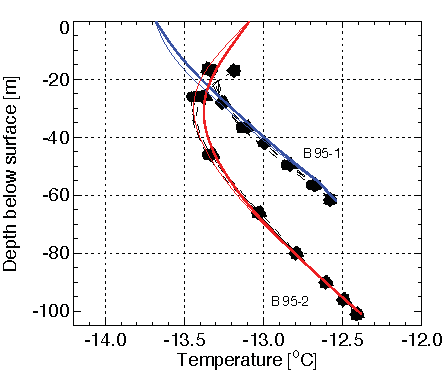
\includegraphics[width=0.49\textwidth]{figures/c_temp_trans_k32}
   \caption{Markers indicate temperatures measured in two boreholes on
the same flow line, $200\unit{m}$ apart, on Colle Gnifetti.  Solid
lines are the results of numerical interpretation of the data with
steady state (left) and transient (right) temperature
evolution. Notice that the different curvature of the steady state
profiles is due to firn density and advection. From
\cite{LuethiFunk2001}.}
 \label{fig:colle-profiles}
\end{figure}

\begin{figure}[p] \centering
 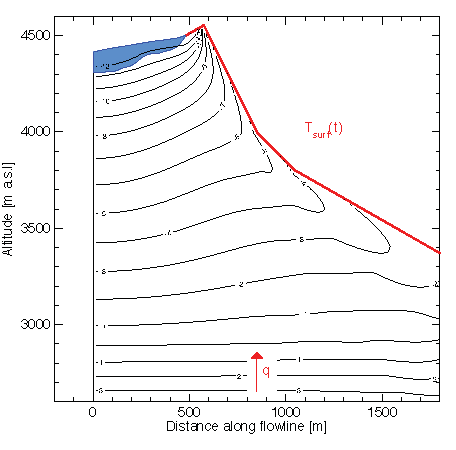
\includegraphics[width=0.49\textwidth]{figures/c_temp_iso_sing_mid}
\hfill
 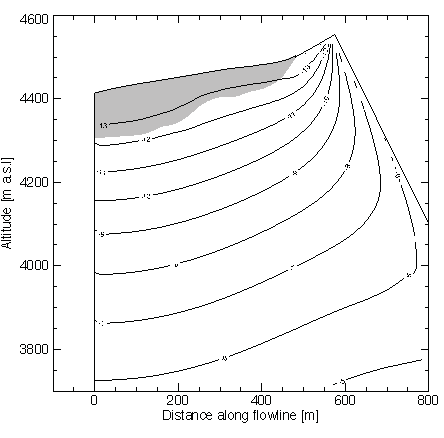
\includegraphics[width=0.49\textwidth]{figures/c_temp_iso_sing_top}
\hfill
 \caption{Modeled temperature distribution within the Monte Rosa
massif.  Notice the highly increased surface temperature on the south
(right) face which leads to horizontal heat fluxes close to steep
mountain faces.  Thawing permafrost at the base of the mountain was
essential to reproduce the measured heat flux at the glacier base.
From \cite{LuethiFunk2001}.}
 \label{fig:colle-moutain}
\end{figure}


Modeling the advection and conduction of heat in a glacier is usually
not sufficient.  The geothermal heat flux close to the glacier base is
affected by the ice temperature, and therefore by the glacier flow,
and the flux of meltwater.  Figure~\ref{fig:colle-moutain} shows the
temperature distribution in whole massif, with the glacier on top.
Notice that there are areas within the mountain where heat flows
horizontally (heat always flows perpendicular to the isotherms).  Heat
flux at sea level was assumed to be $70\unit{mW}\unit{m}^{-2}$, but it
had to be greatly reduced to match the observed fluxes.  In the model
this was accomplished with freezing/thawing ice within the rock
(permafrost), which is a reaction to climate changes since the last
ice age.  The lowest calculated permafrost margin was at about
$2900\unit{m}$ elevation.


\section{Temperate ice}
\label{sec:temperate-ice}

In temperate ice, the liquid water fraction $\omega$, replaces $u$:
\begin{equation}
  \label{eq:water-content-equation} \rho L\left(\frac{\partial
\omega}{\partial t} + \mathbf{ v}\cdot\nabla \omega\right) = -\nabla \cdot
\mathbf{ q} + Q,
\end{equation} where $L$ is latent heat of fusion, and $u$ and
$\omega$ are related by $u=\omega L$. Specifying the non-advective
flux $q$ is less straight-forward than for cold ice. Both Fick-type
and Darcy-type diffusion closures haven been proposed. Generally it is
assumed to be small, and often set to zero.

\subsection{Temperate glaciers}
\label{sec:temperate-glaciers}

Liquid water, generated from melting snow or direct input from
rainfall, is routed down{-}glacier by supraglacial streams. When such
streams intersect vertical shafts (moulins), crevasses or fractures,
water can enter the macroscopic englacial water system (MWS,
Figure~\ref{fig:mws}a) mainly formed by a network of decimeter size,
hydraulically connected fractures which can route macroscopic volumes
of water to the bed of the glacier
\citep{FountainWalder1998,Fountain2005}.
%

Water in glaciers occurs also in a fundamentally different system
unconnected from MWS: the microscopic water system (mWS,
Figure~\ref{fig:mws}b). mWS is formed by small ($\mu m$) water
inclusions found in veins along three grain intersections, lenses on
grain boundaries and in irregular shapes
\citep{RaymondHarrison1975,Nye1989,Mader1992,FountainWalder1998}. Such
water inclusions are primarily generated in the accumulation area
where meltwater percolates in the porous firn and become part of the
glacier-ice crystalline structure when pores closed for compaction
\citep{Paterson1971,Lliboutry1976,Pettersson2004}.


In a temperate glacier, all heat that is produced at the boundaries or
within the glacier is used to melt ice. This meltwater then becomes
part of mWS. The water content, however, is small, usually between 0.1
and 4 volume percent.  The water is stored in veins and triple
junctions between the ice grains, where it can slowly percolate
through the ice matrix if veins are not blocked by air bubbles.  The
water between ice grains has an important effect on the deformation
properties of ice, and it affects the rate factor $A$ in Glen's flow
law \citep{Duval1977,Paterson1994}
%
\begin{align}
 \label{eq:ratefactor-water} A(\omega) &= (3.2 + 5.8 \omega) \cdot
10^{-15} \unit{kPa}^{-3}\unit{s}^{-1} \notag\\ &= (101 + 183\omega)
\unit{MPa}^{-3}\unit{a}^{-1}\,,
\end{align}
%
where $\omega$ is the percentage of water within the ice (also called
moisture content or liquid water fraction).
%
Temperate glacier ice is a mixture of ice ($97-99\unit{\%}$), water
($1-3\unit{\%}$), and small amounts of air and minerals.  For pure ice
the melting temperature $T_m$ depends on absolute pressure $p$ by
%
\begin{equation}
 \label{eq:clausius-pure} T_m = T_{tp} - \gamma\, (p -
p_{\text{tp}})\,,
\end{equation}
% 
where $T_{tp}=273.16\unit{K}$ and $p_{tp}=611.73\unit{Pa}$ are the
triple point temperature and pressure of water.  The
Clausius-Clapeyron constant is $\gamma_{p}= 7.42 \cdot 10^{-5}
\unit{K}\unit{kPa}^{-1}$ for pure water/ice.  Since glacier ice is not
pure, the value of $\gamma$ can be as high as $\gamma_a = 9.8 \cdot
10^{-5} \unit{K}\unit{kPa}^{-1}$ for air saturated water
\citep{Harrison1975a}.


 \begin{figure}[tbhp] \centering
  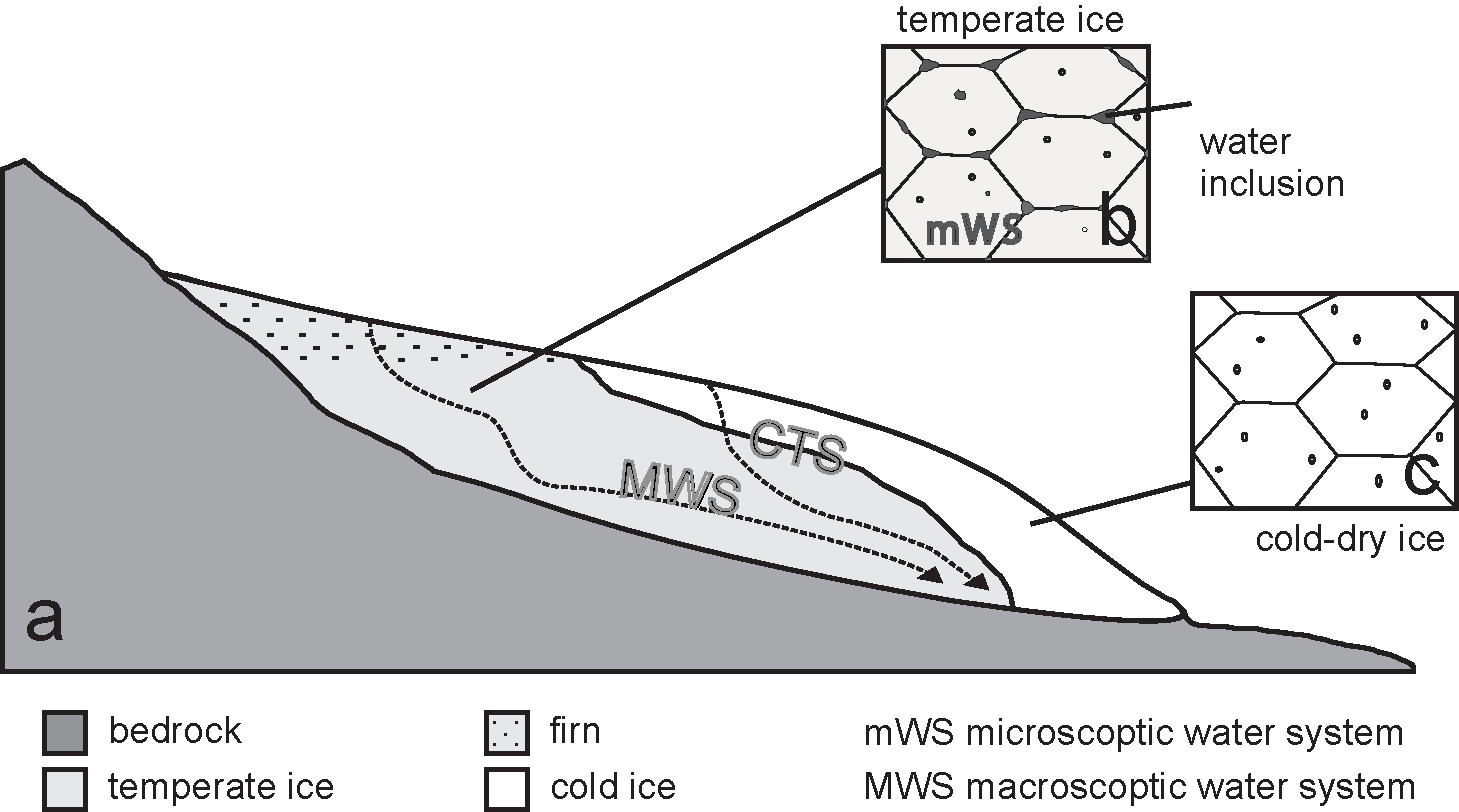
\includegraphics[width=12.cm]{figures/mws}
  \caption{Illustration of macroscopic water system (MWS) and
microscopic water system (mWS) found in the temperate ice. The
cold-temperate transition surface (CTS) is the englacial boundary
separating temperate ice (b) from the cold ice (c). Modified after
\cite{Gusmeroli2010}}
  \label{fig:mws}
\end{figure}


\section{Polythermal glaciers and ice sheets}
\label{sec:polythermal-glaciers}

Polythermal glaciers occur in different climates and at different
geographic locations. Given the winter cooling of the surface layer in
temperate glaciers, or the summer warming of the surface layer in cold
glaciers, most glaciers are seasonally polythermal. The only
exceptions are perhaps cold glaciers in the extremely cold climate of
Antarctica. Considering only perennial polythermal glaciers, the most
frequent structures are the so-called Scandinavian-type and
Canadian-type polythermal glaciers
(Figure~\ref{fig:thermal-structures}).

\begin{figure}
  \begin{centering}
  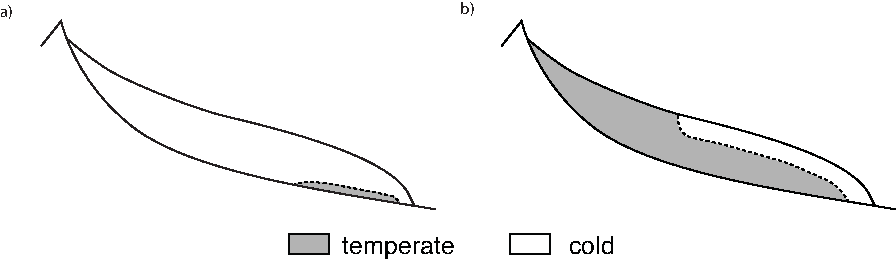
\includegraphics[width=\textwidth]{figures/CTSstructures-2land}
  \caption{Longitudinal section of glaciers with (a) Canadian-type and
(b) Scandinavian-type polythermal structures.}
  \label{fig:thermal-structures}
  \end{centering}
\end{figure}

The Scandinavian type occurs in Svalbard \citep{Bamber1988,Jania1996},
Scandinavia \citep{HolmlundEriksson1989}, the Rocky Mountains
\citep{Paterson1971}, Alaska and the Antarctic Peninsula
\citep{Breuer2006}. Such glaciers are mostly temperate except for a
cold surface layer in the ablation zone. This seemingly paradoxical
situation may be explained by the summer heat input, which is stored
due to percolation of meltwater into the upper firn area, whereas this
heat is lost due to runoff of meltwater over the impermeable surface
ice in the ablation zone (Figure~\ref{fig:scandinavian-structure}). If
winter temperatures increase, the cold layer thins and may eventually
disappear, leaving an entirely temperate glacier.

 \begin{figure} \centering
   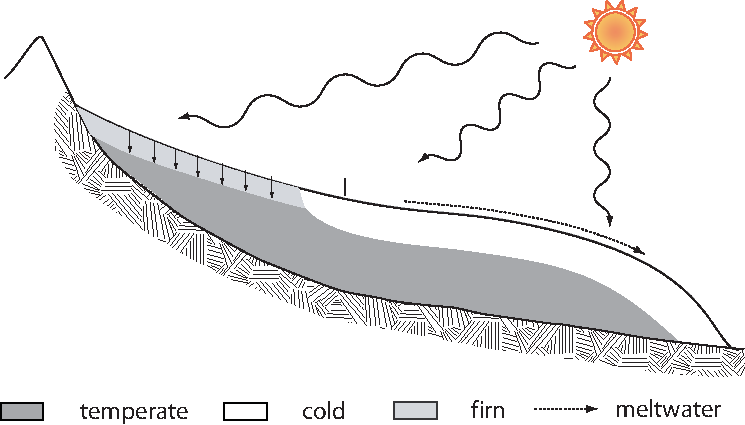
\includegraphics[width=12cm]{figures/CTS_scandic}
   \caption{Scandinavian-type polythermal structure. Most of the ice
is temperate (gray color) except for a cold near-surface layer in the
ablation zone. The summer heat input is stored due to percolation of
meltwater into the upper firn area, whereas this heat is lost due to
runoff of meltwater over the impermeable surface ice in the ablation
zone.}
   \label{fig:scandinavian-structure}
 \end{figure}

%
The Canadian type occurs at high Arctic latitudes in Canada
\citep{Blatter1987,Blatter1988} and Alaska, but the large ice sheets
in Greenland and Antarctica also show this polythermal structure
locally. Canadian-type glaciers are mostly cold except for a temperate
layer at the bed in the ablation zone. The temperate layer at the
bedrock can be of considerable thickness and is due to geothermal heat
flux and heat dissipation due to friction and ice deformation.  The
latter is highest close to the base because stresses and strain rates
are highest there.  Depending on the climate, ice thickness and ice
flow, the thickness of this basal layer may shrink to zero, leaving a
so-called basal hot spot \citep{Classen1971}. There may be additional
polythermal structures, such as combinations of the above if glaciers
span an extreme altitude range, or at confluences of glaciers with
different thermal structures \citep{Eisen2009}.


Gorner-/Grenzgletscher is the biggest polythermal glacier in the Alps.
Cold ice originating from Colle Gnifetti is advected down to the
confluence area at $2500\unit{m}\unit{a.s.l.}$, and all the way to the
glacier tongue.  Figure \ref{fig:temp-profile-gorner} shows the slow
cooling of a borehole in the confluence area after hot-water drilling.
The cold ice is mostly impermeable to water which leads to the
formation of deeply incised river systems and surficial lakes which
sometimes drain through crevasses or \emph{moulins}.


\begin{figure}[tbhp] \centering
 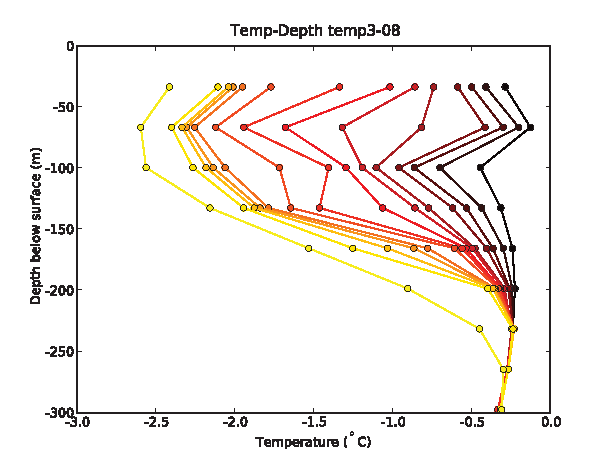
\includegraphics[width=0.6\textwidth]{figures/gorner-temp-depth_temp3-08}
 \caption{Cooling of a borehole drilled in the confluence area of
Gorner-/Grenzgletscher. Temperatures measured every day after
completion of drilling are shown in increasingly lighter colors, and
after three months (leftmost yellow curve). Data from
\cite{Ryser2009}.
   \label{fig:temp-profile-gorner}}
\end{figure}

Polythermal glaciers are usually cold in their core and temperate
close to the surface and at the bedrock.  Heat sources at the surface
are from the air (sensible heat flux), direct solar radiation (short
wave), thermal radiation (long wave), and the penetration and
refreezing of melt water (convection and latent heat).

Nice examples of the polythermal structure of the Greenland ice sheet
are the temperature profiles in Figure \ref{fig:jako-temp-profiles},
measured in Jakobshavn Isbr\ae{}, Greenland
\citep{IkenEchelmeyer1993,Funk1994a,Luethi2002}.  The drill sites are
located $50\unit{km}$ inland of the margin of the Greenland ice sheet,
at a surface elevation is $1100\unit{m} \unit{a.s.l.}$, where ice
thickness on the ice sheet is $830\unit{m}$, but about $2500\unit{m}$
in the ice stream center.


\begin{figure}[tbhp] \centering
 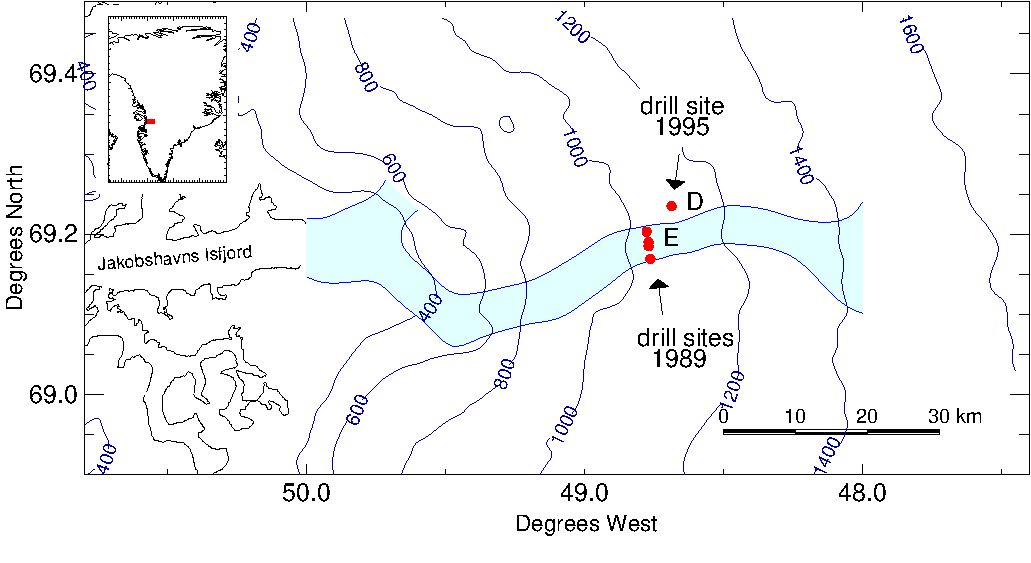
\includegraphics[width=\textwidth]{figures/jako_map.pdf} \\[2em]
 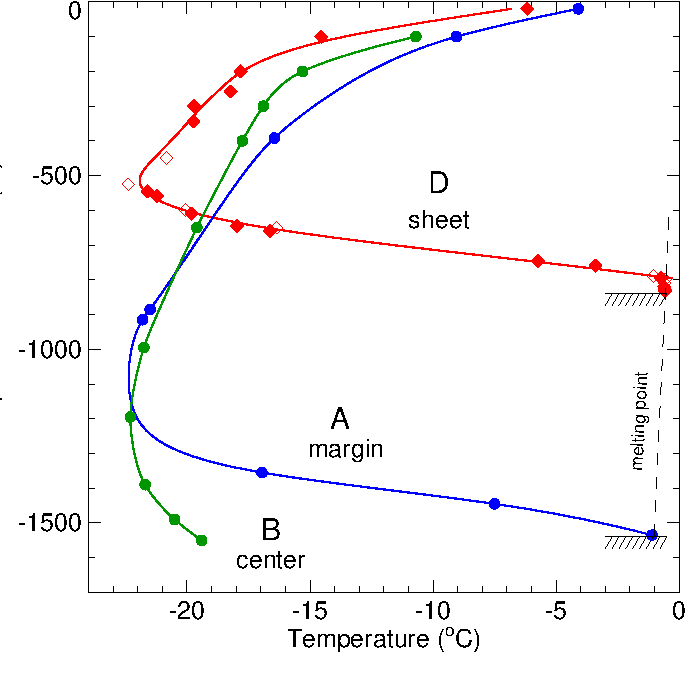
\includegraphics[width=0.49\textwidth]{figures/jako_temp_bed.pdf}
 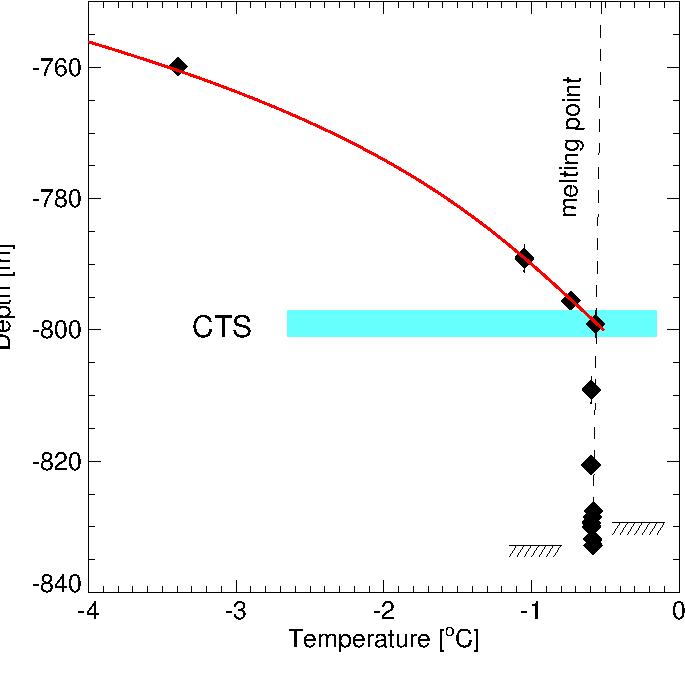
\includegraphics[width=0.49\textwidth]{figures/jako_temp_bed100.pdf}
 \caption{Top: Location map of the drill sites on Jakobshavn Isbr\ae,
Greenland, where temperature profiles have been measured.  Left:
Profile A is from the southern side of the ice stream, profile B from
the center (the ice is about $2500 \unit{m}$ thick there) and D on the
northern margin.  Notice the basal temperate ice at D and also at A.
The very cold ice in the middle of the profiles is advected and is
slowly warming up.  Right: Closeup of the $31\unit{m}$ thick temperate
layer at site D. The cold-temperate transition surface CTS is at
freezing conditions. The Clausius-Clapeyron gradient (dashed line) is
$\gamma = 0.0743 \unit{K}\unit{MPa}^{-1}$.  From \cite{Luethi2002}.
 \label{fig:jako-temp-profiles}}
\end{figure}

\begin{figure}[tbhp] \centering
 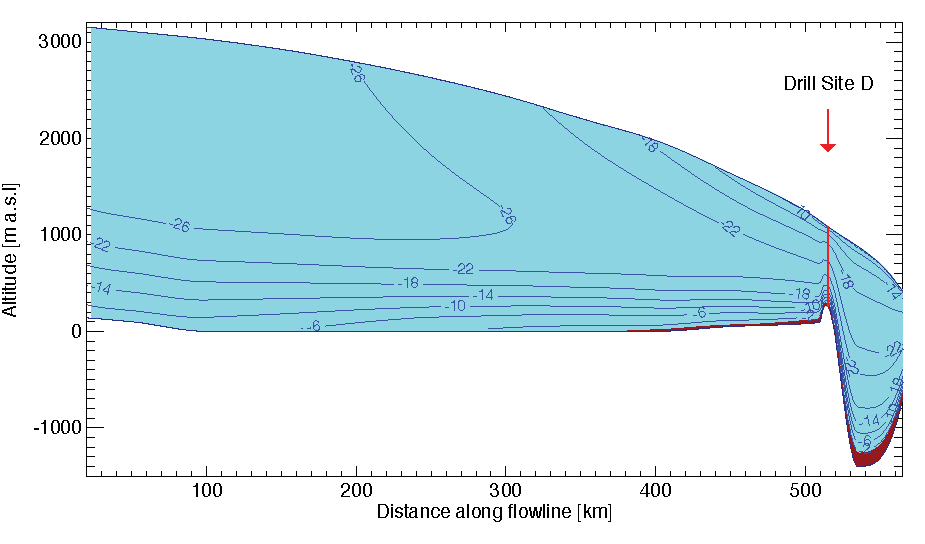
\includegraphics[width=\textwidth]{figures/jako_mod_temp_cont_all_slide}\\[2em]
 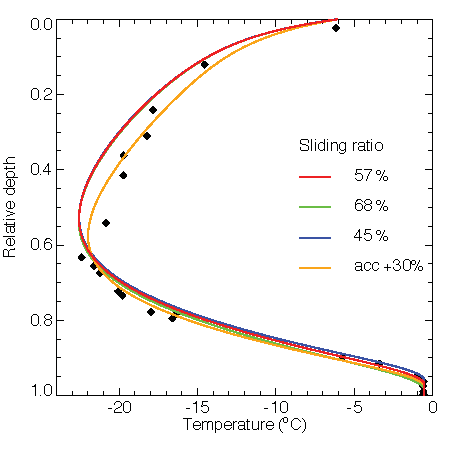
\includegraphics[width=0.49\textwidth]{figures/jako_mod_temp_profs}\hfill
 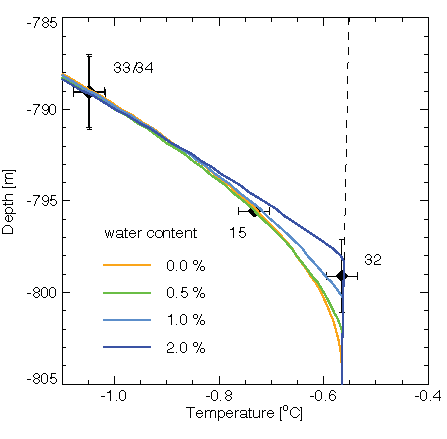
\includegraphics[width=0.49\textwidth]{figures/jako_temp_bed_mod_CTS}
 \caption{Top: Temperature distribution along a flow line in the
Greenland Ice Sheet, and passing through drill site D.  Clearly
visible is the advection of cold ice and the onset of a basal
temperate layer far inland at $380\unit{km}$.  Left: Modeled
temperature profiles for different ratios of basal motion.  Right:
Modeled temperature profiles for different values of the water content
in the temperate ice.  From \cite{Funk1994a} and \cite{Luethi2002}.
 \label{fig:jako-temp-model}}
\end{figure}

In Figure \ref{fig:jako-temp-profiles} (bottom left) temperatures are
highest close to the surface and close to the bed. The thick, very
cold layer in between is advected from the inland parts of the ice
sheet (see Figure \ref{fig:jako-temp-model} top).  The lowest
$31\unit{m}$ are at the pressure melting temperature $T_m =
\cels{-0.55}$.  A quick calculation with Equation
(\ref{eq:clausius-pure}), and reasonable values for the ice density
and gravity gives
%
\begin{align}
 \label{eq:jako-melting-point} T_m&= T_{tp} - \gamma_p (p -
p_{\text{tp}}) = T_p - \gamma_{p} (\rho g H - p_{tp}) \notag\\ &=
273.16 \unit{K} - 7.42 \cdot 10^{-5} \unit{K}\unit{kPa}^{-1} \left(
900\unit{kg}\unit{m}^3 \cdot 9.825\unit{m}\unit{s}^{-2}\cdot
830\unit{m} \right) \notag\\ &\simeq 273.16 \unit{K} - 0.545\unit{K}
\simeq 272.615 \unit{K} = \cels{-0.54}\,.
\end{align}
%
The strong curvature of the temperature profiles where they are
coldest indicates that the ice is warming.  Upward heat flux from the
temperate zone close to the base is very high.  The temperature
gradient just above the CTS ($800\unit{m}$ depth) in profile D is
$0.048\unit{K}\unit{m}^{-1}$. The upward heat flux therefore is (per
unit area)
%
\begin{equation}
 \label{eq:jako-heat-flux} Q \;=\; k \,\ddz{T} \;\simeq\;2.1
\unit{W}\unit{m}^{-1}\unit{K}^{-1} \cdot 0.048 \unit{K}\unit{m}^{-1}
\;\simeq\; 0.1\unit{W}\unit{m}^{-2}\,.
\end{equation}
%
This heat has to be produced locally, since heat fluxes in the
temperate zone below $800\unit{m}$ depth are downward (away from the
CTS), but very small due to the Clausius-Clapeyron temperature
gradient.  The only way to produce this heat is by freezing the water
contained within the temperate ice.  From a flow model we know that
the CTS moves with respect to the ice by $v_\text{freeze} \sim 1
\unit{m}\unit{a}^{-1}$.  With a moisture content of $\omega =
1\unit{\%}$ (by volume) we obtain a heat production rate of
%
\begin{align}
 \label{eq:jako-heat-production-cts} P &= \omega\,v_\text{freeze}\,
\rho_w L \;\simeq \; 0.01 \cdot 1 \unit{m}\unit{a}^{-1} \cdot 1000
\unit{kg}\unit{m}^3 \cdot 3.33\cdot 10^5\unit{J}\unit{kg}^{-1}
\notag\\ &= 3.55 \unit{MJ}\unit{a}^{-1}\unit{m}^{-3} \simeq 0.113
\unit{W}\unit{m}^{-3}
\end{align}
% 
which matches up nicely with the heat transported away by diffusion
(Eq.~\ref{eq:jako-heat-flux}).  A detailed analysis with the flow
model shows that the most likely value for the water content is about
$1.5\unit{\%}$ (Fig.~\ref{fig:jako-temp-model}, bottom right).
Another interesting result form the model is that an ice column
passing through drill site D has already lost the lowest $40\unit{m}$
through melting at the glacier base.

\section{An enthalpy formulation for glaciers and ice sheets}

To model polythermal ice masses, ideally one would solve the
temperature equation (Eq.~\ref{eq:temperature-equation}) in cold ice
and the water content equation (Eq.~\ref{eq:water-content-equation})
in temperate ice, and applying Stefan-type matching conditions at the
CTS. The CTS is a free boundary in such models and may be treated with
front-tracking methods.  Because they require an explicit
representation of the CTS as a surface, however, such methods are
somewhat cumbersome to implement.

Enthalpy methods describe the CTS as a level set of the enthalpy
variable.  No explicit surface-representation scheme is required and
no \emph{a priori} restrictions apply to CTS shape.  Transitions
between thermal structures caused by changing climatic conditions can
be modeled even if nontrivial CTS topology arises at intermediate
stages.

The specific enthalpy is often defined as $E = U + p/\rho$ where $U$
is the specific internal energy and $p$ is the pressure.  (Note $E$
and $U$ have SI units $\text{J}\,\text{kg}^{-1}$.) Here we use
``enthalpy'' synonymous with ``internal energy'', $E=U$, because we do
not include the work associated with changing the volume, namely the
$p/\rho$ term in the specific (per volume) case. The functional
relationships between enthalpy, liquid water fraction, and temperature
is given by
\begin{align}
\label{eq:temp-from-enthalpy} T(E,p) &= \begin{cases} T_{\text i}(E),
& E < E_{\text s}(p), \\ T_{\text m}(p), & E_{\text s}(p) \le E,
        \end{cases} \\
\label{eq:omega-from-enthalpy} \omega(E,p) &= \begin{cases} 0, & E <
E_{\text s}(p), \\ L^{-1} ( E-E_\text{s}(p) ), & E_{\text s}(p) \le E,
        \end{cases}
\end{align} where $E_{\text{s}}(p)$ is the enthalpy of $\omega=0$ ice
at the pressure-melting temperature $T_{\text{m}}(p)$. Schematic plots
of temperature and water content as functions of enthalpy are shown in
Figure~\ref{fig:enthalpy-function}, with points $E_{\text s}$ and
$E_{\text l}(p) = E_{\text w}(T_{\text m}(p),p) = E_{\text s}(p) + L$
noted.  Equations \eqref{eq:temp-from-enthalpy} and
\eqref{eq:omega-from-enthalpy} will only be applied to cold or
temperate ice (mixtures), and therefore $E<E_{\text l}(p)$ in all
cases.

\begin{figure} \centering{ \begin{tikzpicture}[>=stealth,scale=7.5]
      \coordinate (origin) at (0,0);
      \coordinate (Hend) at +(1,0);
      \coordinate (Tend) at +(0,0.5);
      \coordinate (Tm) at +(0,0.2);
      \coordinate (Hs) at ( $ (origin)!0.2!(Hend) $ );
      \coordinate (Hl) at ( $ (origin)!0.7!(Hend) $ );
      \coordinate (TmHs) at (0.2,0.2);
      \coordinate (TmHl) at (0.7,0.2);
      \coordinate (omega) at ( $ (origin)!0.9!(Hend) $ );
     \draw[->] (origin) -- (Hend) node[anchor=north] {$E$};
      \draw[->,densely dotted] (omega) -- +(0,0.5) node[anchor=west] {$\omega$};
      \draw[->] (origin) -- (Tend) node[anchor=east] {$T$};
      \draw[dashed] (Hs) node[anchor=north] {$E_{\text s}$} -- +(0,0.45);
      \draw[dashed] (Hl) node[anchor=north] {$E_{\text l}$} -- +(0,0.45);
      \draw[dashed] (Tm) node[anchor=east] {$T_{\text m}$} -- +(1,0);
      \draw[thick] (origin) -- (TmHs) -- (TmHl) -- +(60:0.2);
      \draw[dotted,thick] (Hs) -- (0.7,0.42) -- +(.22,0) node[anchor=west] (one) {1} ;
\end{tikzpicture}
 }
  \caption{At fixed pressure $p$ the temperature of the ice/liquid
water mixture is a function of enthalpy, $T=T(E,p)$ (solid line), as
is the liquid water fraction, $\omega=\omega(E,p)$ (dotted line).
Points $E_{\text s}(p)$ and $E_{\text l}(p)$ are the enthalpy of pure
ice and pure liquid water, respectively, at temperature $T_{\text
m}(p)$.}
  \label{fig:enthalpy-function}
\end{figure}

We can then write the enthalpy balance equation as
\begin{equation}
  \label{eq:energy-balance} \rho \left(\ddt{E} + \bv \cdot \grad
E\right) = - \Div \bq + Q
\end{equation} with
\begin{equation}\label{eq:enthalpy-flux} {\mathbf q} = \left\{
    \begin{array}{rl} - K_{\text i}(E)\, \nabla E, & \qquad
\text{cold},\\ - k(E,p) \nabla T_{\text m}(p) - K_0 \nabla E, & \qquad
\text{temperate},
    \end{array} \right.
\end{equation} where $K_{\text{i}}$ and $K_0$ are the enthalpy
diffusivity of cold and temperate ice, respectively, and $k$ is the
heat conductivity expressed in terms of enthalpy.

In writing the above enthalpy equations, we have assumed that we're
dealing with incompressible ice. It is, however, important to note
that the enthalpy framework is more general, and can be easily
extended to the compressible case.  Because the enthalpy equation is
the same type of partial differential equation as the temperature
equation, rendering an existing numerical model polythermal is quite
straigth-forward. As so often, the devil lies in specifying the
boundary conditions. For a comprehensive (and lengthy) discussion of
an enthalpy formulation for glaciers and ice sheets, see
\cite{Aschwanden2012}.


\newpage \bibliography{thermobib}


\end{document}